\section{離散フーリエ変換}

離散フーリエ変換とは,時系列空間の離散データ$f(t)$を周波数空間の離散データ$F(\omega)$へ
変換する手法であり,式(\ref{eq:dft})で定義される.
\begin{align}
  F(\omega) = \sum_{t=0}^{N-1} f(t) e^{-j \frac{2 \pi \omega}{N} t} \label{eq:dft}
\end{align}
このとき,式(\ref{eq:dft})における$N$は$f(t)$におけるデータ数である.


\begin{figure}[h]
  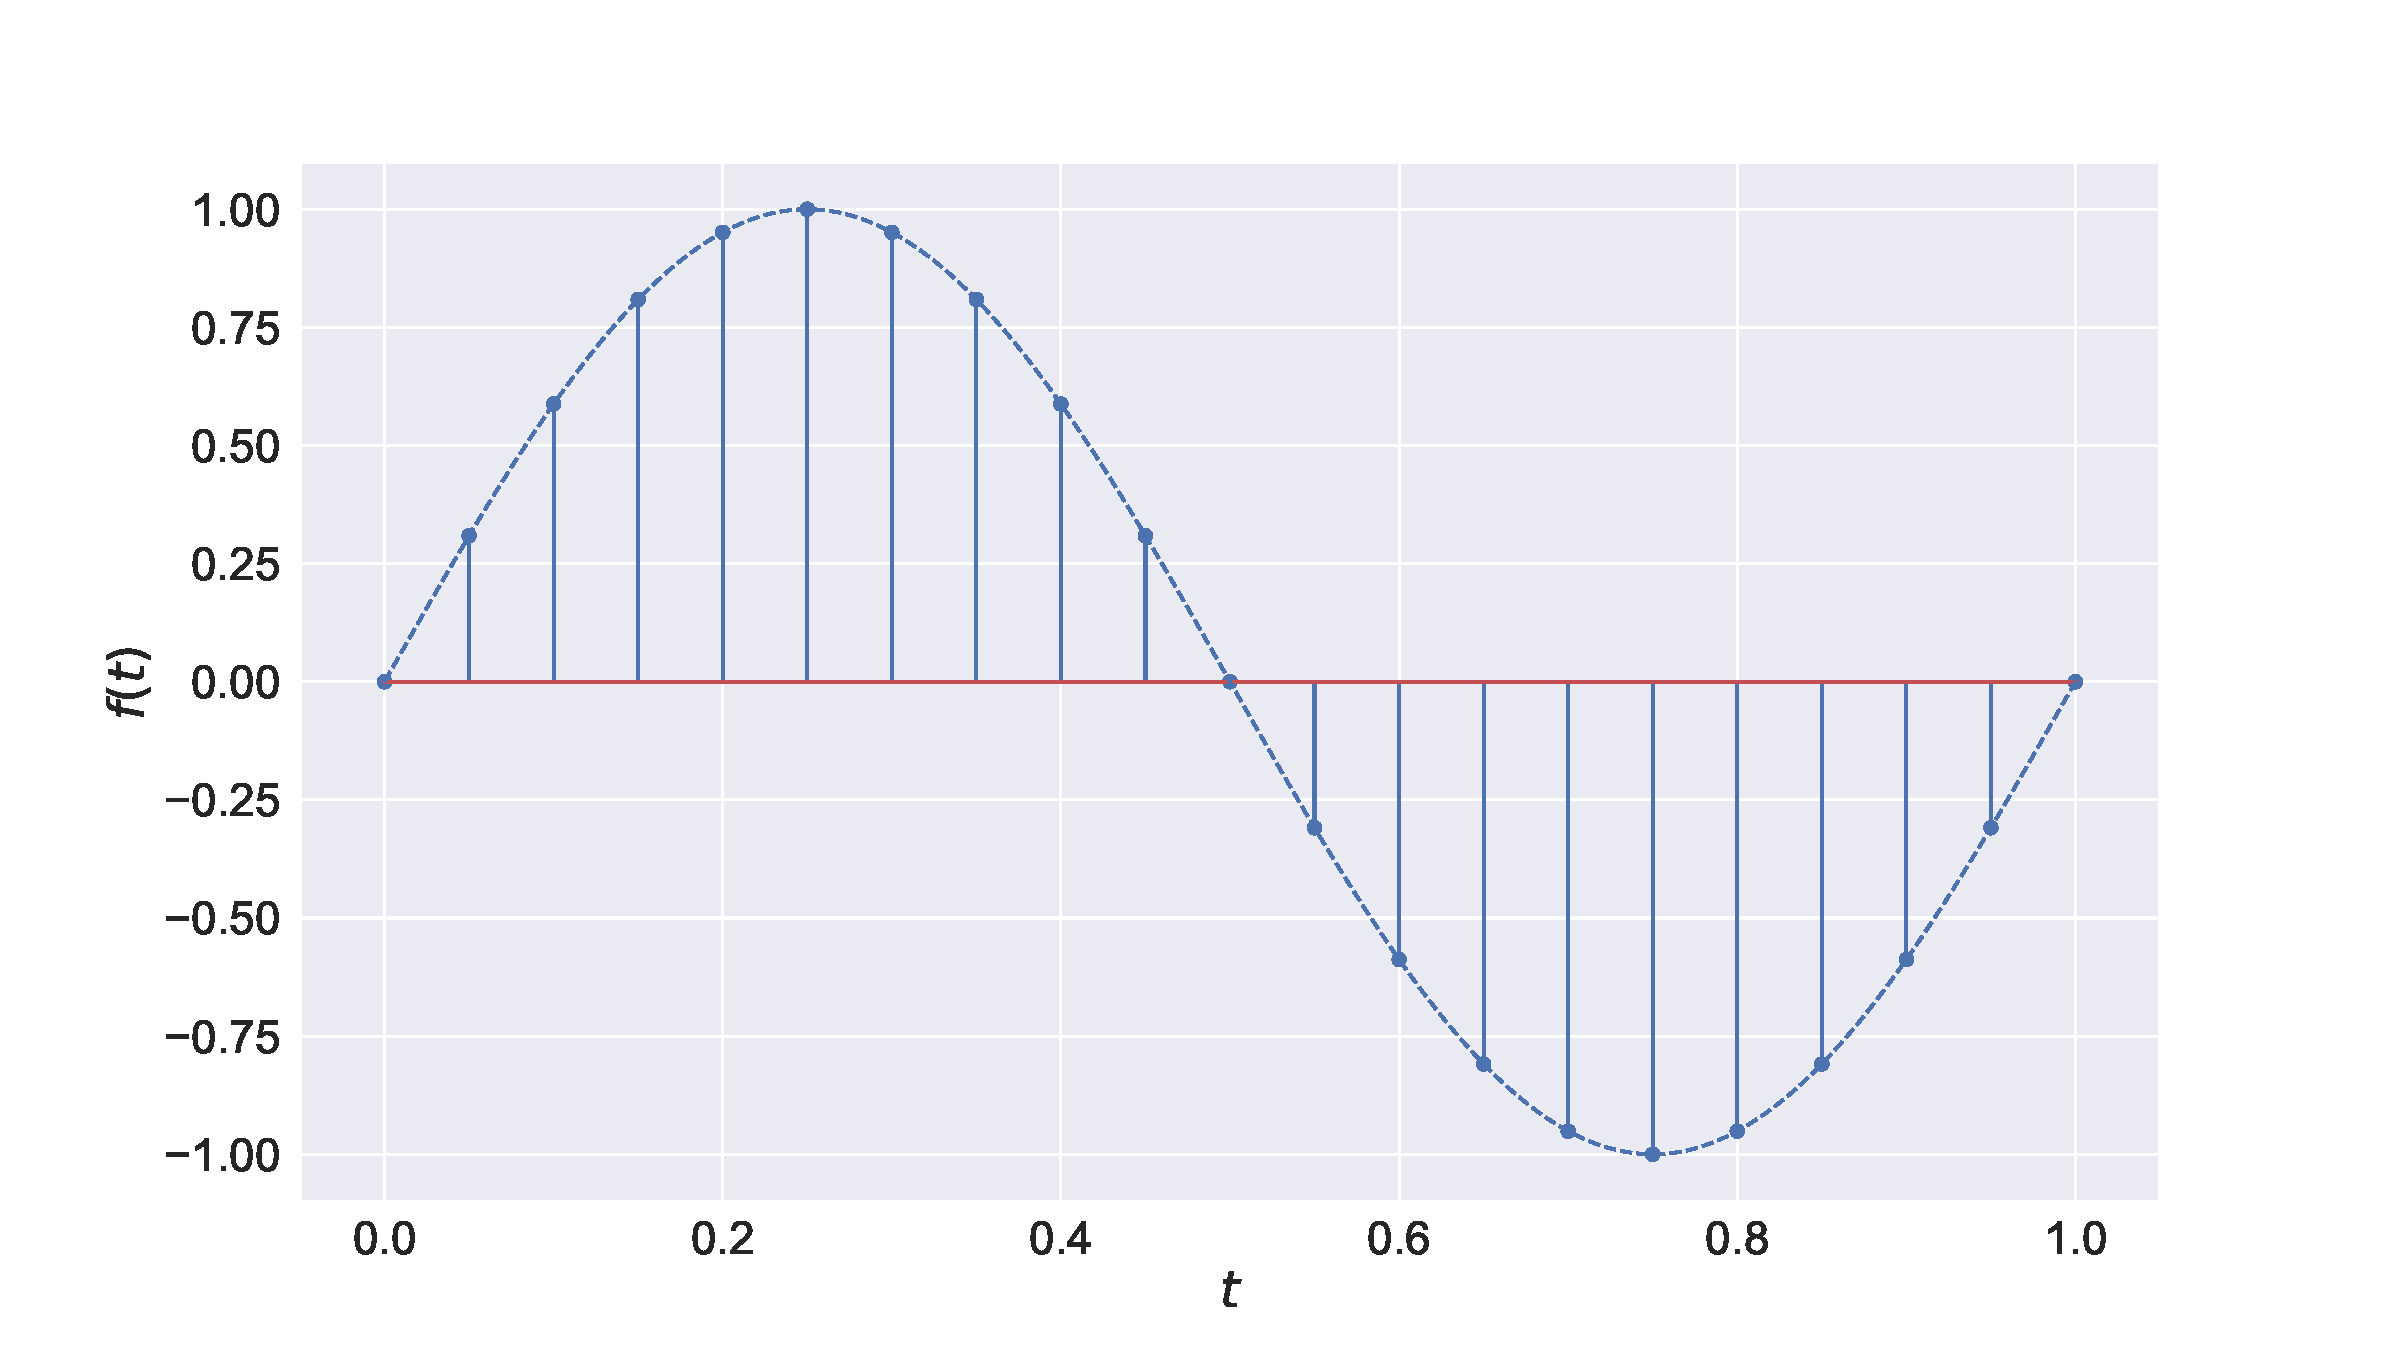
\includegraphics[clip, width=\textwidth]{figure/sin.pdf}
  \caption{$\sin (2 \pi t)$の離散データ}
\end{figure}

\begin{figure}[h]
  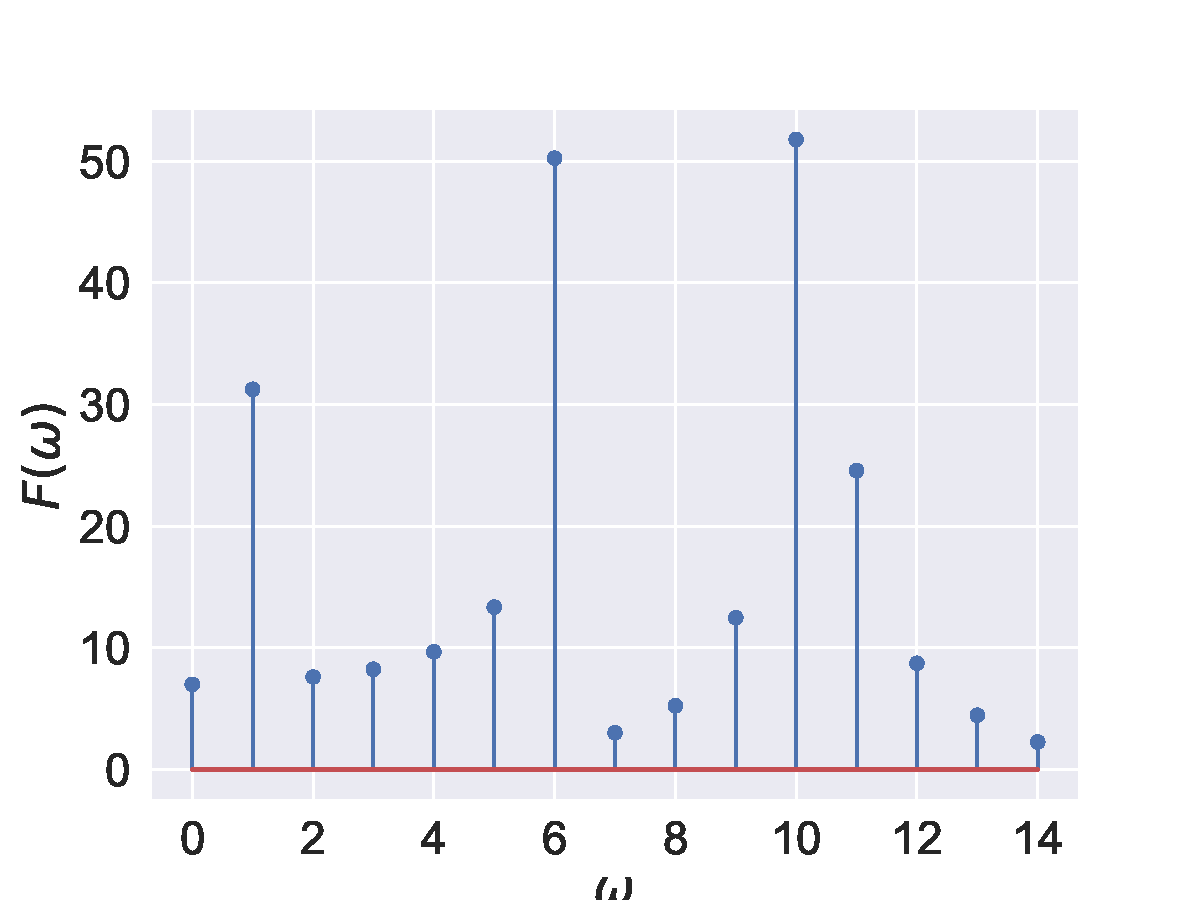
\includegraphics[clip, width=\textwidth]{figure/sin_dft.pdf}
  \caption{$\sin (2 \pi t)$の周波数空間における離散データ}
\end{figure}
